\chapter{Special Functions and Useful Formulas}

\section{Special Functions}

\subsection{Hyperbolic Functions}
The hyperbolic functions are defined as follows:
\begin{align}
    \sinh x & = \frac{\ee^x - \ee^{-x}}{2} \\
    \cosh x & = \frac{\ee^x + \ee^{-x}}{2} \\
    \tanh x & = \frac{\sinh x}{\cosh x} = \frac{\ee^x - \ee^{-x}}{\ee^x + \ee^{-x}}
\end{align}

The diagram below shows the graphs of the hyperbolic functions $\sinh x$, $\cosh x$ and $\tanh x$.
\begin{figure}[h!]
    \centering
    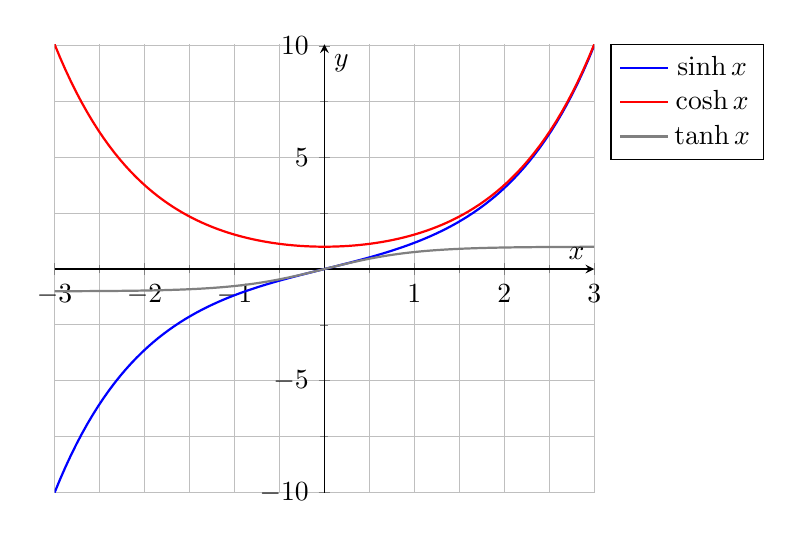
\begin{tikzpicture}
        \begin{axis}[
            axis lines = center,
            xlabel = {$x$},
            ylabel = {$y$},
            domain=-3:3,
            samples=100,
            legend pos=outer north east,
            grid=both,
            minor tick num=1,
        ]
        \addplot [blue, thick] {sinh(x)};
        \addlegendentry{$\sinh x$}
        
        \addplot [red, thick] {cosh(x)};
        \addlegendentry{$\cosh x$}
        
        \addplot [gray, thick] {tanh(x)};
        \addlegendentry{$\tanh x$}
        \end{axis}
    \end{tikzpicture}
    \caption{Graphs of Hyperbolic Functions}
    \label{fig:hyperbolic_functions}
\end{figure}

From whis we can easily see that $\cosh x$ is even function while $\sinh x$ and $\tanh x$ are odd functions. The domain of $\sinh x$ and $\cosh x$ is $(-\infty, +\infty)$ while the domain of $\tanh x$ is $(-\infty, +\infty)$ but the range is $(-1, 1)$. There are more useful identities involving hyperbolic functions:
\begin{align}
    \cosh^2 x - \sinh^2 x & = 1 
\end{align}
This can be proved easily by plugging in the definitions of $\sinh x$ and $\cosh x$. Also the derivatives of hyperbolic functions are:
\begin{align}
    \frac{\dd}{\dd x} \sinh x & = \cosh x \\
    \frac{\dd}{\dd x} \cosh x & = \sinh x \\
    \frac{\dd}{\dd x} \tanh x & = \frac{1}{\tanh^2 x} x
\end{align}
Additiaonally, the double-angle formulas are:
\begin{align}
    \sinh 2x & = 2 \sinh x \cosh x \\
    \cosh 2x & = \cosh^2 x + \sinh^2 x = 2 \cosh^2 x - 1 = 1 + 2 \sinh^2 x \\
    \tanh 2x & = \frac{2 \tanh x}{1 + \tanh^2 x}
\end{align}
angle sumation and half-andgle formulas are 
\begin{align}
    \sinh (x \pm y) & = \sinh x \cosh y \pm \cosh x \sinh y \\
    \cosh (x \pm y) & = \cosh x \cosh y \pm \sinh x \sinh y \\
    \tanh (x \pm y) & = \frac{\tanh x \pm \tanh y}{1 \pm \tanh x \tanh y} \\
    \sinh \frac{x}{2} & = \pm \sqrt{\frac{\cosh x - 1}{2}} \\
    \cosh \frac{x}{2} & = \pm \sqrt{\frac{\cosh x + 1}{2}} \\
    \tanh \frac{x}{2} & = \frac{\sinh x}{\cosh x + 1} = \frac{\cosh x - 1}{\sinh x}
\end{align}



\clearpage
\chapter{Group Theory Basics} \label{chap:GroupTheory}
 

\section{Definition of a Group}

\begin{definition}[Group]
    Let $G$ be a set on which a binary operation $G \times G \ra G$ is defined. $G$ is called a group iff the followind holds:
    \begin{itemize}
        \item \emph{Associativity}: $(g_1 \cdot g_2) \cdot g_3 = g_1 \cdot (g_2 \cdot g_3), \forall g_1, g_2, g_3 \in G$
        \item \emph{Identity Element}: There exists an element $e \in G$ such that $e \cdot g = g \cdot e = g, \forall g \in G$
        \item \emph{Inverse Element}: For each $g \in G$, there exists an element $g^{-1} \in G$ such that $g \cdot g^{-1} = g^{-1} \cdot g = e$
    \end{itemize}
\end{definition}
\begin{ex}
    \begin{itemize}
        \item
        \item The integers $\Z$ form a group with respect to the binary operation of addition, denoted by $(\Z,+)$. The unit element is given by $0$, and the inverse of $n$ is $-n$, $\forall n \in \Z$.
        \item The integers $\Z$ are not a group with respect to the binary operation of multiplication, denoted by $(\Z, \times)$. This is because not every element has an inverse in $\Z$; for example, there is no integer $m$ such that $2 \times m = 1$.
        \item The rotation group of 3d space $O(3) = \left\{O \in M_3(\R)\right\}$\footnote{$M_n(\cdot)$ denotes a $n \times n$ matrix with entries from the set in the parentheses.} with respect to the binary operation of matrix multiplication is a group. The unit element is given by the identity matrix $I_3$, and the inverse of a rotation matrix is its transpose.
    \end{itemize}
\end{ex}

\begin{definition}[Basic definitions:]
    \begin{itemize}
        \item A group $G$ is called \emph{finite, discrete} or \emph{continuous} depending on whether the set $G$ is finite, discrete (isomorphic to $\Z$) or uncountable.
    \end{itemize}
\end{definition}



\section{Lie Algebra, Lie Group, Basics of representation theory}
For translations, the generator is the momentum operator $\op$, which commutes with itself in different directions, i.e.,
\begin{align}
    \comm{\op_i}{\op_j} = 0 \quad \text{for } i,j = x,y,z
\end{align}
For rotations, the generator is the angular momentum operator $\oL$, which does not commute with itself in different directions, i.e.,
\begin{align}
    \comm{\oL_i}{\oL_j} = \ii \hbar \epsilon_{ijk} \oL_k \quad \text{for } i,j,k = x,y,z
\end{align}
\begin{definition}[Lie Algebra]
    \begin{enumerate}
        \item A Lie algebra $\mathfrak{g}$ is a real vector space. 
        \item Within $\mathfrak{g}$, there exists a bilinear, scew-symmetric map 
    \end{enumerate}
\end{definition}



\section{Representations of a Group} \label{sec:GroupRepresentations}






\chapter{Spherical Harmonics}

\section{Agular Momentum in Spherical Coordinates}

\subsection{General Expressions} \label{sec:AngularMomentum_SphericalCoord}
The Cartesian coordinates $(x,y,z)$ of a vector $\bfvec{r}$ are related to its spherical coordinates $(r,\theta,\phi)$ by 
\begin{align}
    x & = r \sin \theta \cos \phi \\
    y & = r \sin \theta \sin \phi \\
    z & = r \cos \theta
\end{align}
The orthonormal basis vectors in spherical coordinates $(\hat{\ee}_ r, \hat{\ee}_ \theta, \hat{\ee}_ \phi)$ are related to those in Cartesian coordinates $(\hat i ,\hat j, \hat k)$ by
\begin{align}
    \hat{\ee}_ r & = \sin \theta \cos \phi \hat i + \sin \theta \sin \phi \hat j + \cos \theta \hat k \\
    \hat{\ee}_ \theta & = \cos \theta \cos \phi \hat i + \cos \theta \sin \phi \hat j - \sin \theta \hat k \\
    \hat{\ee}_ \phi & = -\sin \phi \hat i + \cos \phi \hat j
\end{align}
Relove these equations, we have
\begin{align}
    \hat i & = \sin \theta \cos \phi \hat{\ee}_ r + \cos \theta \cos \phi \hat{\ee}_ \theta - \sin \phi \hat{\ee}_ \phi \\
    \hat j & = \sin \theta \sin \phi \hat{\ee}_ r + \cos \theta \sin \phi \hat{\ee}_ \theta + \cos \phi \hat{\ee}_ \phi \\
    \hat k & = \cos \theta \hat{\ee}_ r - \sin \theta \hat{\ee}_ \theta
\end{align}
Differentiating these equations, we obtain
\begin{align}
    \dd \hat{\ee}_ r & = \hat{\ee}_ \theta \dd \theta + \hat{\ee}_ \phi \sin \theta \dd \phi \\
    \dd \hat{\ee}_ \theta & = -\hat{\ee}_ r \dd \theta + \hat{\ee}_ \phi \cos \theta \dd \phi \\
    \dd \hat{\ee}_ \phi & = -\hat{\ee}_ r \sin \theta \dd \phi - \hat{\ee}_ \theta \cos \theta \dd \phi
\end{align}
From these, we can derive the component derivatives in spherical coordinates:
\begin{align}
    \pdv{r}{x} & = \sin \theta \cos \phi, & \pdv{r}{y} & = \sin \theta \sin \phi, & \pdv{r}{z} & = \cos \theta \\
    \pdv{\theta}{x} & = \frac{\cos \theta \cos \phi}{r}, & \pdv{\theta}{y} & = \frac{\cos \theta \sin \phi}{r}, & \pdv{\theta}{z} & = -\frac{\sin \theta}{r} \\
    \pdv{\phi}{x} & = -\frac{\sin \phi}{r \sin \theta}, & \pdv{\phi}{y} & = \frac{\cos \phi}{r \sin \theta}, & \pdv{\phi}{z} & = 0
\end{align}
From these we can find 
\begin{align}
    \pdv{}{x} & = \sin \theta \cos \phi \pdv{}{r} + \frac{\cos \theta \cos \phi}{r} \pdv{}{\theta} - \frac{\sin \phi}{r \sin \theta} \pdv{}{\phi} \\
    \pdv{}{y} & = \sin \theta \sin \phi \pdv{}{r} + \frac{\cos \theta \sin \phi}{r} \pdv{}{\theta} + \frac{\cos \phi}{r \sin \theta} \pdv{}{\phi} \\
    \pdv{}{z} & = \cos \theta \pdv{}{r} - \frac{\sin \theta}{r} \pdv{}{\theta}
\end{align}

Such that the gradient, Laplacian, is clear to be expressed 
\begin{align}
    \nabla = \hat i \pdv{}{x} + \hat j \pdv{}{y} + \hat k \pdv{}{z} = \hat{ee}_r \pdv{}{r} + \hat{\ee}_ \theta \pdv{}{\theta}
\end{align}
\section{Basics of Spherical Harmonics}


\section{Associated Legendre Functions} \label{sec:AssociatedLegendreFunctions}





